\documentclass[a4paper, 12pt]{article}

\usepackage{geometry}
\geometry{left=2cm, right=2cm, top=2cm, bottom=2cm}

\usepackage{cmap}
\usepackage{mathtext} 
\usepackage[T2A]{fontenc}
\usepackage[utf8]{inputenc}
\usepackage[english,russian]{babel}	

\usepackage{amsfonts,amssymb,amsthm,mathtools}
\usepackage{amsmath}
\usepackage{icomma} 

\usepackage{graphicx} 
\graphicspath{{picturies/}}
\usepackage{wrapfig}

\usepackage{array,tabularx,tabulary,booktabs}
\usepackage{longtable}
\usepackage{multirow}

\usepackage{caption}
\captionsetup{labelsep=period}

\renewcommand{\phi}{\varphi}
\newcommand{\eps}{\varepsilon}
\newcommand{\parag}[1]{\paragraph*{#1:}}

\newcounter{Points}
\setcounter{Points}{1}
\newcommand{\point}{\arabic{Points}. \addtocounter{Points}{1}}

\author{Радькин Кирилл, Б01-005}
\date{15.04.22}
\title{Лабораторная работа 4.3.1. Изучение дифракции света.}

\begin{document}
\maketitle
\thispagestyle{empty}
\newpage

\textbf{В работе используются:} оптическая скамья, ртутная лампа, монохроматор, щели с регулируемой шириной, рамка с вертикальной нитью, двойная щель, микроскоп на поперечных салазках с микрометрическим винтом, зрительная труба.

\section*{А. Дифракция Френеля}

\textbf{Теоретическая справка:}

\begin{itemize}
    \item Суммарная ширина $m$ зон Френеля $z_m$ определяется соотношением:
    
    \begin{equation*}
        z_m = \sqrt{a m \lambda}
    \end{equation*}
\end{itemize}

\textbf{Схема установки:}

\begin{figure}[!h]
    \centering
    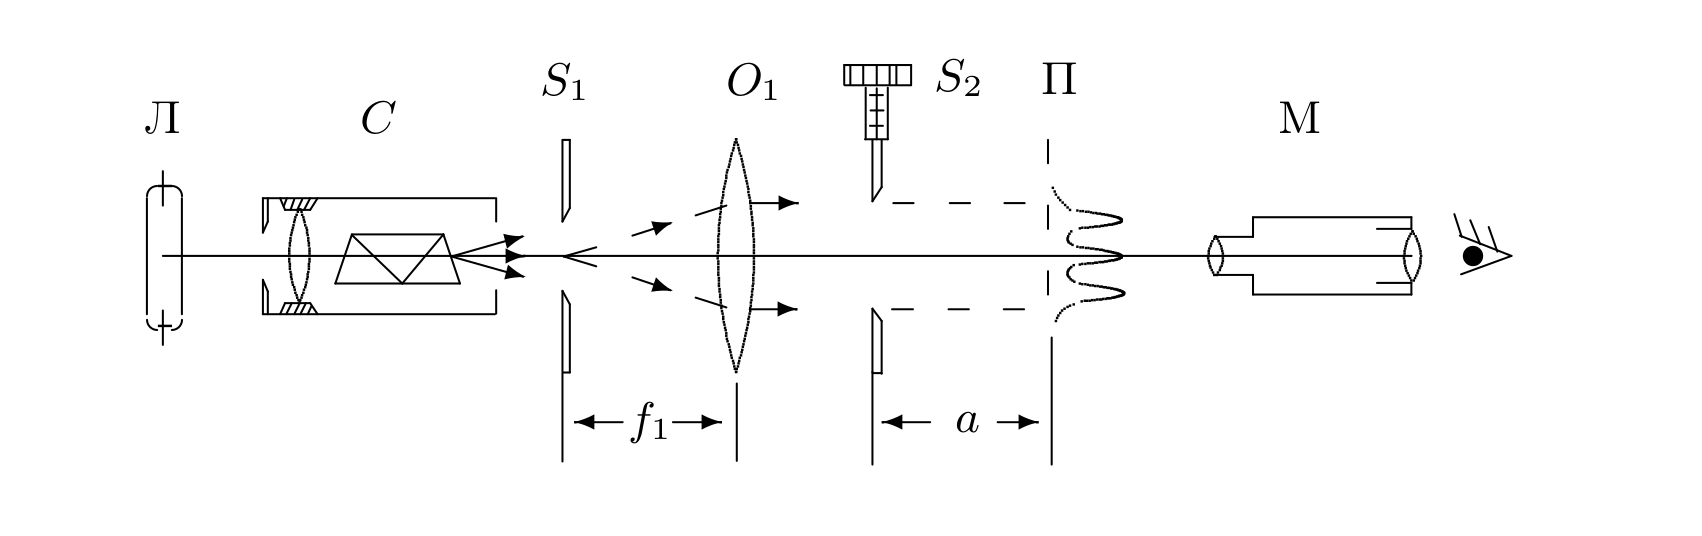
\includegraphics[scale = 0.3]{pic1.png}
    \caption{Схема установки для наблюдения дифракции Френеля}
    \label{pic1}
\end{figure}

\textbf{\\Ход работы:}

\begin{enumerate}
    \item Настроим зрительную трубу на бесконечность, соберем установку.
    \item Определим нуль микрометрического винта щели: $0.053 \pm 0.001$ мм
    \item Сфокусируем микроскоп на щель
    \item Запишем: начальное положение микроскопа~---~$52.8$ см, положение второй диафрагмы~---~$69$ см
    \item Отодвинем микроскоп до того момента, пока на фоне щели не появится одна темная полоса. Далее, приближая микроскоп к щели, снимем зависимость количества темных полос от координаты микроскопа.
    
    \begin{tabular}{|c|c|c|c|c|c|} \hline
        n & 1 & 2 & 3 & 4 & 5 \\ \hline
        $l, $ см & 50.1 & 50.8 & 51.3 & 51.6 & 51.8 \\ \hline
    \end{tabular}

    \item Измерим ширину щели с помощью микроскопа: $0.32 \pm 0.02$ мм. Сравним с показаниями микрометрического винта щели: $0.037 \pm 0.01$ мм. Сильный расхождений не обнаружено.
    \item Закрепим микроскоп на оптической скамье и пронаблюдаем, что при уменьшении щели количество полос уменьшается.
    \item Рассчитаем величину $2z_m$ и построим график $2z_m = f(m)$ и отложим на графике величину $D$:
    
    
    \begin{figure}[!h]
        \centering
        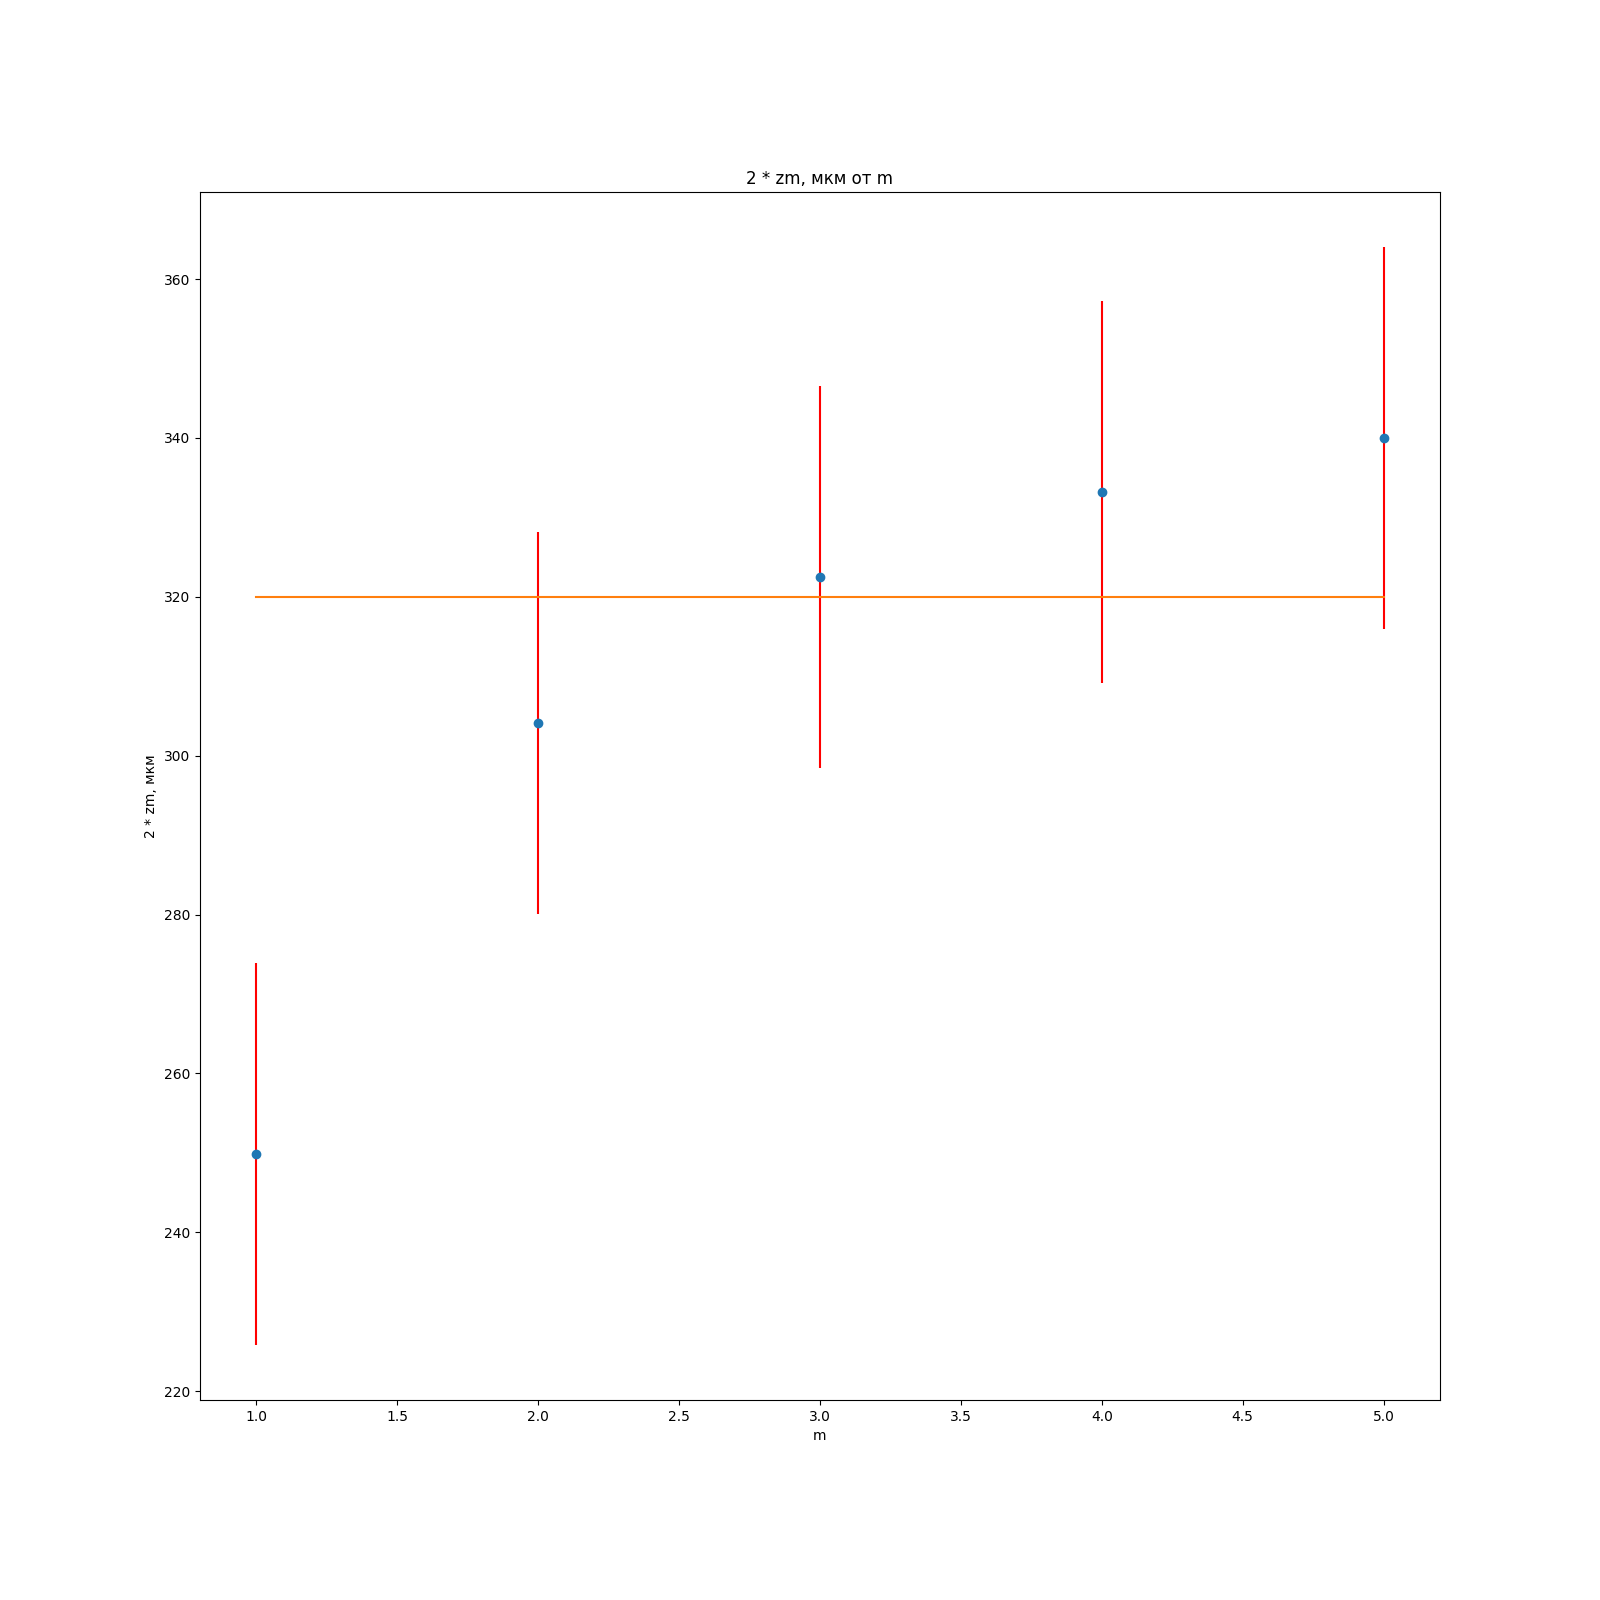
\includegraphics[scale=0.4]{graph1.png}
        \caption{График ширины зон Френеля от $m$}
        \label{graph1}
    \end{figure}
\end{enumerate}

\section*{Б. Дифракция Фраунгофера на щели}

\textbf{Теоретическая справка:}

\begin{itemize}
    \item Расстояние $X_m$ темной полосы от оптической оси объектива $O_2$ пропорционально фокусному расстоянию $f_2$:
    \begin{equation*}
        X_m = f_2 m \dfrac{\lambda}{D}
    \end{equation*}
\end{itemize}

\newpage

\textbf{Схема установки:}
\begin{figure}[!h]
    \centering
    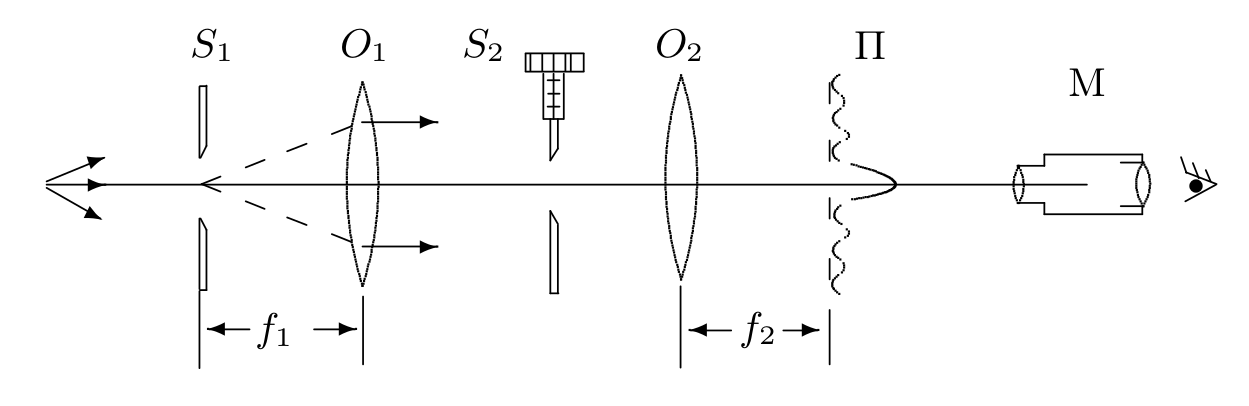
\includegraphics[scale=0.3]{pic2.png}
    \caption{Схема установки для дифракции Фраунгофера}
    \label{pic2}
\end{figure}

\textbf{Ход работы:}

\begin{enumerate}
    \item Для перехода к дифракции Фраунгофера добавим к установке на рис. \ref{pic1} линзу $O_2$
    \item Настроим установку
    \item Измерим с помощью винта поперечного перемещения микроскопа координаты $X_m$ нескольких дифракционных минимумов (от $-m$ до $+m$).
    
    \begin{tabular}{|c|c|c|c|c|c|} \hline
        $m$ & -2 & -1 & 0 & 1 & 2 \\ \hline
        $X_m$, мм & 1.46 & 1.6 & 1.9 & 2.16 & 2.34 \\ \hline 
    \end{tabular}

    Определим ширину $D$ щели $S2$: $D = 0.39 \pm 0.01$ мм

    Запишем фокусное расстояние линзы $O_2$: $F_2 = 12.5$ см

    \item Построим график $X_m$ от $m$ (рис. \ref{graph2}):
    
    \begin{figure}[!h]
        \centering
        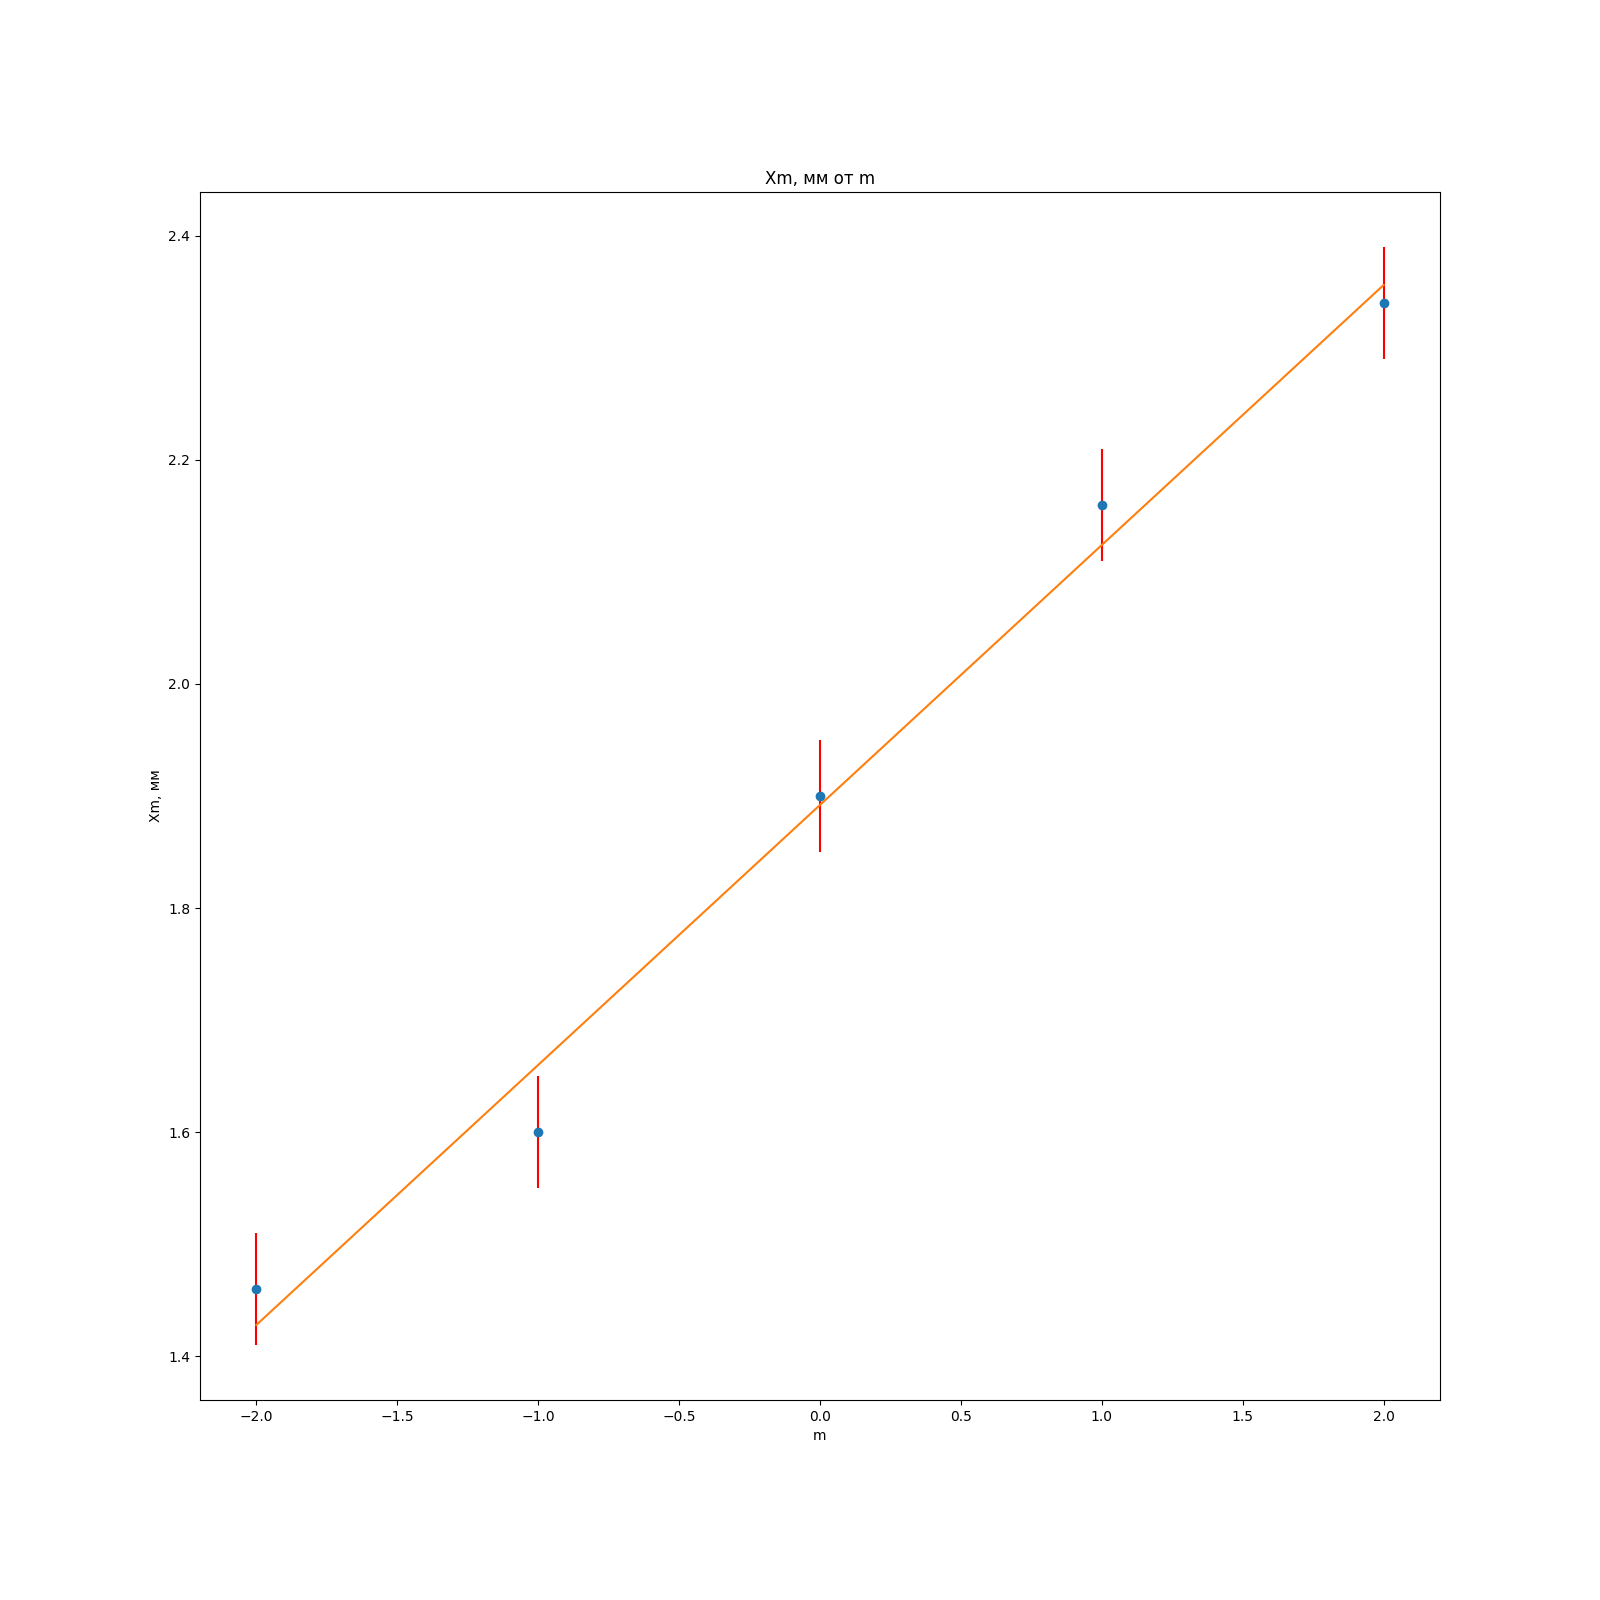
\includegraphics[scale=0.4]{graph2.png}
        \caption{График $X_m$ от $m$}\
        \label{graph2}
    \end{figure}

    \item По углу наклона прямой определим среднее расстояние между соседними минимумами: $\Delta X = 0.23 \pm 0.01$
    \item Рассчитаем ширину щели: $D = 0.311 \pm 0.020$ мм, сравним с измеренным значением: $D_{изм} = 0.385 \pm 0.10$ мм. Расхождения результатов $\approx 11 \%$
\end{enumerate}

\section*{В. Дифракция Фраунгофера на двух щелях}

\textbf{Теоретическая справка:}

\begin{itemize}
    \item Линейное расстояние $\delta x$ между соседними интерференционными полосами в плоскости П равно:
    
    \begin{equation*}
        \delta x = f_2 \dfrac{\lambda}{d}
    \end{equation*}

    \item Число интерференционных полос, укладывающихся в области центрального дифракционного максимума:
    
    \begin{equation*}
        n = \dfrac{2 \lambda f_2}{D} \dfrac{1}{\delta x} = \dfrac{2 d}{D}
    \end{equation*}

    \item При дифракции света на двух щелях чёткая система интерференционных полос наблюдается только при достаточно узкой ширине входной щели $S$. При увеличении её ширины интерференционная картина периодически пропадает и появляется вновь, но полосы при этом оказываются сильно размытыми и видны плохо. Это явление объясняется наложением интерференционных картин от разных элементов широкой щели $S$.
    Первое размытие интерференционных полос возникает при условии:

    \begin{equation*}
        \dfrac{b}{f_1} = \dfrac{\lambda}{d}
    \end{equation*}
\end{itemize}

\newpage

\textbf{Схема установки:}

\begin{figure}[!h]
    \centering
    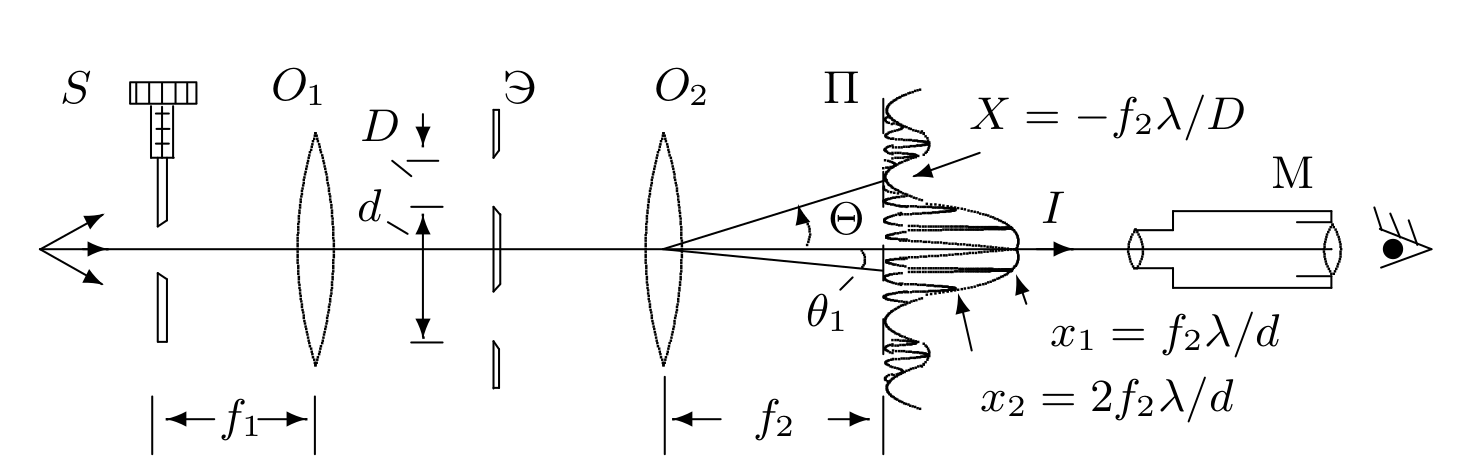
\includegraphics[scale=0.3]{pic3.png}
    \caption{Схема установки для наблюдения дифракции Фраунгофера на двух щелях}   
    \label{pic3} 
\end{figure}

\textbf{Ход работы:}

\begin{enumerate}
    \item Настроим установку
    \item Определим с помощью микрометрического винта поперечных салазок микроскопа координаты самых удалённых друг от друга тёмных полос внутри центрального максимума: левая полоса~---~$2.28$ мм, правая полоса~---~$2.68$ мм. Просчитаем число светлых промежутков между ними: 10. Измерим ширину центрального максимума:$0.4$ мм.
    \item Для исследования влияния простраственной когерентности на видность интерференционной картины. Для этого подберем такую ширину $b_0$ щели $S$, при которой наступает первое исчезновение интерференционных полос: $b_0 = 1.9$ мм.
    \item Запишем фокусные расстояния обеих линз: $F_1 = 9$ см, $F_2 = 12.5$ см.
    \item Определим расстояние $\delta x$ между минимумами по результам измерений: $\delta x = 0.04$ мм. 
    \item Рассчитаем величину $d$: $d = 1.8 \pm 0.1$ мм, сравним с измеренной $d_{изм} = 2.1$ мм. Разница $\approx 16 \%$
\end{enumerate}

\section*{Г. Влияние дифракции на разрешающую способность оптического инструмента}

\textbf{Теоретическая справка:}

\begin{itemize}
    \item Критерий Рэлея:
    
    \begin{equation*}
        \dfrac{\lambda}{D_0} = \dfrac{d}{f_1}
    \end{equation*}
\end{itemize}

\newpage

\textbf{Схема установки:}

\begin{figure}[!h]
    \centering
    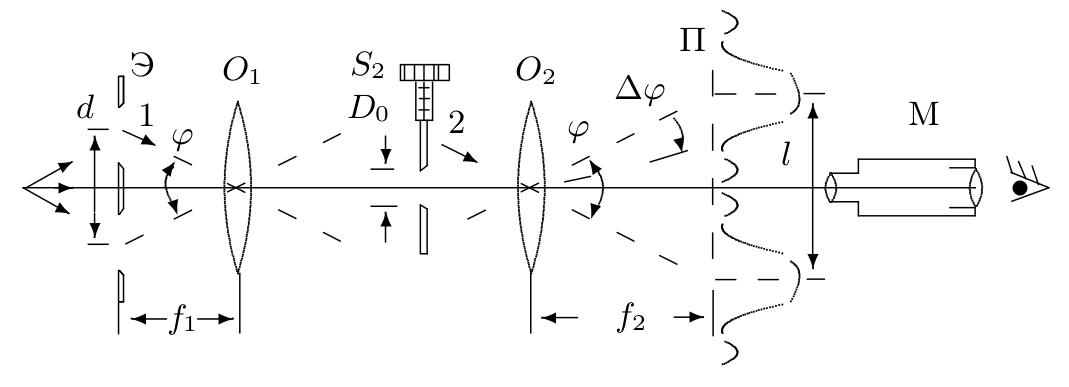
\includegraphics[scale=0.3]{pic4.png}
    \caption{Схема установки для исследования разрешающей способности оптического инструмента}
    \label{pic4}
\end{figure}

\textbf{Ход работы:}

\begin{enumerate}
    \item Соберем схему согласно рис. \ref{pic4}
    \item Поставим между линзами щель и, уменьшая ее ширину, подберем ее так, чтобы изображения обоих щелей почти сливались, но все-таки были различимы и запишем показания микрометрического винта: $0.94$ момента
    \item Поставим двойную щель перед микроскопом, сделаем чертеж щели и запишем координаы каждой из вертикалей:
    
    \begin{figure}[!h]
        \centering
        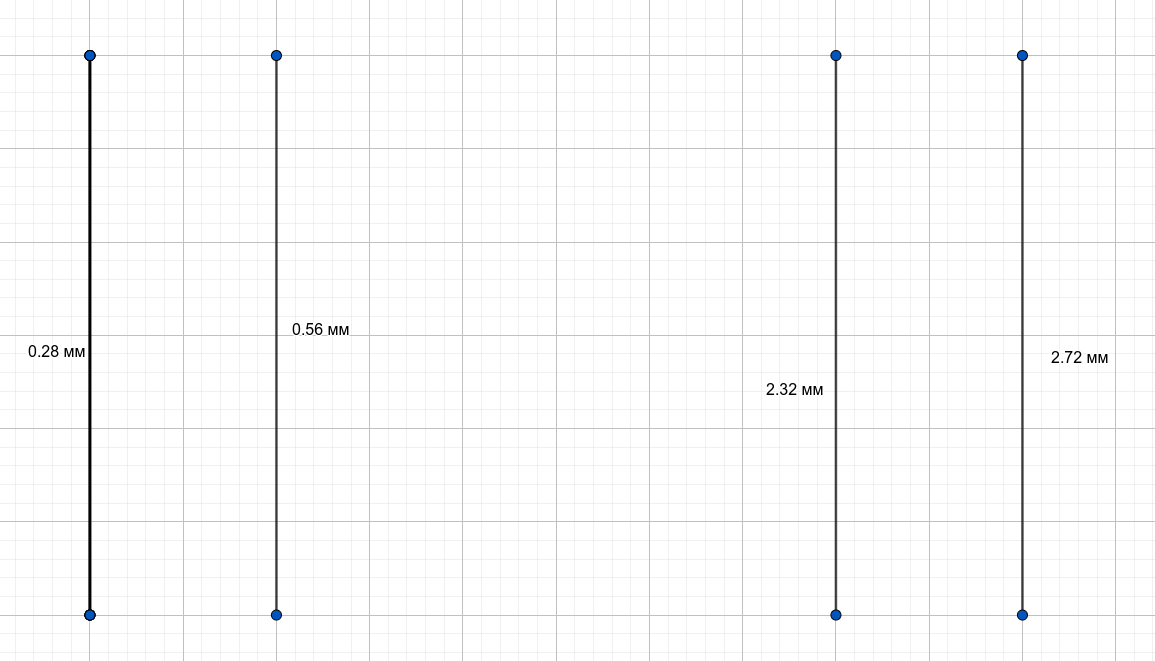
\includegraphics[scale=0.3]{pic5.png}
        \caption{Координаты вертикалей}
        \label{pic5}
    \end{figure}

    \item Для проверик справедливости критерия Рэлея, сравним измеренную ширину щели $D_0$ с расчетом по формуле: $D_0 = \dfrac{\lambda f_1}{d} = 0.0288$ мм
\end{enumerate}

\end{document}